%!TEX root = ../Report.tex
\chapter{Development Plan}
\label{devplan}

\section{Scope}
Please refer to the Project Scope section [\ref{projscope}] for details.

\section{Project Planning and Oversight}
This project will be planned and managed using a tool called Trello \cite{trello}. Columns are used to specify the status of each work item referred to as a `card'. Each card describes the task that needs to be completed. Checklists can be added to a card in order to plan the work breakdown and check things off as they are completed. Dr. Mateti and I are both members of this board and can be assigned to different cards in order to specify who needs to work on certain items. Each card has a conversation functionality where we can both add comments in order to communicate about the work completed and provide updates. When a card is updated, each of us receives an email and mobile notification. \\\\
The columns are `To Do', `In Progress', `Ready for Review', `Done', and `Postponed'. \\\\
I added cards into the `To Do' column at the onset of this project in order to make sure that I had goals for myself to reach. I broke the project down into six milestones. These depicted progress made on the technical report. Every other week, an updated draft is due. I specified those due dates on each card. As Dr. Mateti discovered items he wanted me to research or perform, he would add cards to the `To Do' column as well. \\\\
When I was ready to pick those items up and begin working on them, I would move the card into the `In Progress' column. Once I completed the task, I would put a comment on the card and move it into `Ready for Review' so that Dr. Mateti was aware that I was finished with the item and needed his feedback. If it was an item that did not need feedback, I would move it straight into the `Done' column. If it required feedback, Dr. Mateti would respond with a comment on the card and I would move the card into a column based on the feedback. If more work needed to be done, I would move the card back into `In Progress'. If Dr. Mateti was happy with the work, I would move that card into `Done' and move on to the next card. \\\\
Dr. Mateti added a column called `Postponed' for items that we had planned to work on at the start of the project. However, we found that we were running out of time and wanted to prioritize other items above certain research labs. Those cards were moved into `Postponed'. If time permits, we will revisit those items, but they are not high priority right now.
\begin{figure}[htb]
  \centering
  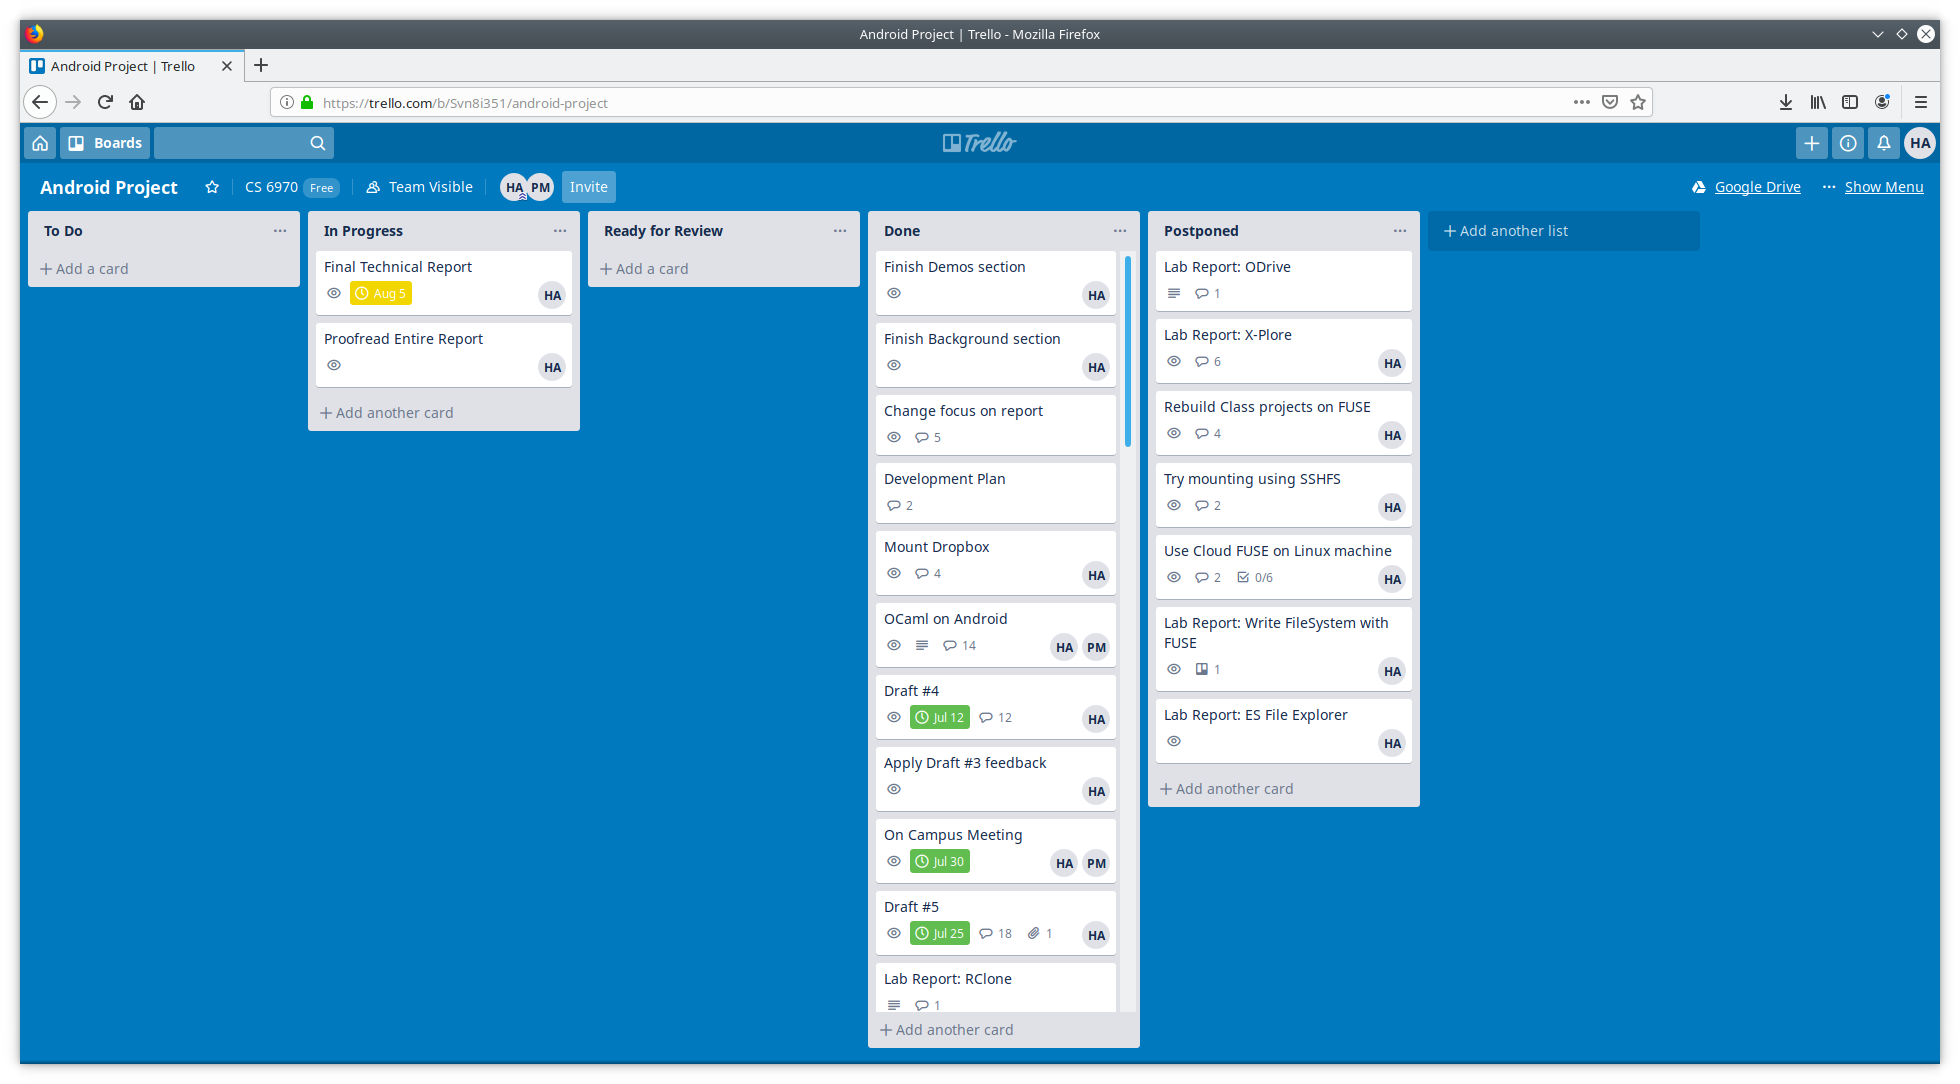
\includegraphics[scale=0.2]{images/trello.png}
  \caption{Trello: Project Management Tool}
  \label{fig:trello}
\end{figure}
\section{Establishing a Software Development Environment}
\begin{enumerate}
\item Setup Linux Operating System
\item Dr. Mateti provided a rooted Nexus 7 tablet
\item Install OCamlFUSE
\item Install Visual Studio Code
\end{enumerate}